\documentclass[a4paper, abstracton, DIV=calc]{scrreprt}

% silence specific warnings
\usepackage{silence}
\WarningFilter{csquotes}{Using preliminary 'polyglossia' interface.}

% fixes certain things for use with XeTeX
\usepackage{xltxtra}

% quotations
\usepackage[strict=true]{csquotes}

% numbers and units
\usepackage{siunitx}

% language support
\usepackage{polyglossia}
\setdefaultlanguage{german}

% line spacing
\usepackage{setspace} 
\setstretch{1.3}

% bibliography
\usepackage[backend=biber, style=alphabetic]{biblatex}
\bibliography{bibliography.bib}

% font stuff
\defaultfontfeatures{Ligatures=TeX}
\setmainfont{Minion Pro}
\setsansfont{Myriad Pro}

% absätze nicht einrücken
\parskip 6pt
\parindent 0pt

% Vermeiden von Schusterjungen und Hurenkindern
\usepackage[all]{nowidow}

% links
\usepackage{hyperref}

% header
% \usepackage{fancyhdr}
% \pagestyle{fancy}

% title page
\author{Sebastian Marr}
\title{Kookkurenzbasierte Link Discovery am Beispiel von Produkttags}

\begin{document}

\maketitle

\begin{abstract}
Durch die Möglichkeit der Benutzerbeteiligung an der Beschreibung, Bewertung und Kategorisierung von Inhalten auf Online-Plattformen werden Begriffswelten aufgebaut, deren Auswertung großes Potenzial für die Verbesserung der Benutzererfahrung bietet. Diese Masterarbeit beschreibt ein Verfahren zum Finden von Zusammenhängen zwischen diesen Begriffen. Grundlage dafür stellen die Daten eines Tagging--Systems und die Ermittlung von Kookkurrenz dar. Die Begriffe und ihre Zusammenhänge werden in eine Graphenrepräsentation transformiert und durch Mining und Integration weiterer Datenquellen angereichert. Zur Priorisierung der Beziehungen für einen Anwendungsfall wird ein Verfahren mittels interaktiver evolutionärer Algorithmen vorstellt und angewendet. Die Ergebnisse der Erzeugung von Beziehungen und der Priorisierung werden präsentiert und schließlich die technische Umsetzung der genannten Verfahren beschrieben.
\end{abstract}

\tableofcontents

\chapter{Einleitung}

Mit der steigenden Menge von nutzergenerierten Inhalten steigt auch die Menge von Metadaten, die mit diesen Inhalten verknüpft sind. Zur späteren Durchsuchbarkeit und Kategorisierung geben viele Online-Plattformen, Marktplätze und Online-Shops ihren Benutzern die Möglichkeit, Inhalte mit Metadaten zu versehen.

Eine oft genutzte Möglichkeit zur Beschreibung von Inhalten sind Tags. Dabei handelt es sich um Wörter oder Wortgruppen, die vom Benutzer frei gewählt werden können, um den Inhalt zu beschreiben. Dabei unterliegt die Eingabe von Tags möglichst wenigen Regeln, um dem Benutzer eine für ihn natürliche Beschreibung des Inhaltes zu ermöglichen. Dabei ist explizit, im Gegensatz zu einer Kategorisierung, die Vergabe von mehreren Tags vorgesehen \cite{sc2005}.

Ein charakteristisches Merkmal von Tags ist dabei, dass sie nur einen bestimmten Aspekt des getaggten Objektes beschreiben. Dabei sind Tags nicht hierarchisch und es werden an keiner Stelle vom Nutzer explizite Zusammenhänge zwischen Tags erstellt. Jedoch liegt die Annahme, dass zwischen Tags Beziehungen herstellbar sind und sich mehrere Tags zu übergeordneten Themen zusammenfassen lassen, nahe. Der Benutzer berücksichtigt diese Beziehungen bei der Eingabe des Tags, formuliert sie jedoch nicht explizit. Die nachträgliche Rekonstruktion der Denkprozesse bei der Eingabe von Tags ist Thema dieser Arbeit.

Dabei ist zu beachten, dass Benutzer bei der Eingabe von Tags unterschiedliche Ziele verfolgen. Idealerweise werden Tags so vergeben, dass sie das getaggte Objekt inhaltlich beschreiben. Jedoch werden vom Benutzer bei der eingabe des Tags weitere Assoziationen hergestellt. Beispielsweise kann der Benutzer mit einem Objekt bestimmte Emotionen oder Wertungen verbinden, die sich in den vergebenen Tags wiederspiegeln.

Auf Marktplätzen, bei denen Verkäufern die Möglichkeit des Taggings ihre Produkte gegeben wird, besteht eine weitere Motivation in der Erhöhung der Auffindbarkeit des Produktes. Dabei kann die inhaltliche Qualität des Tags außer Acht gelassen werden, wenn bei Vergabe einer falschen Beschreibung die Sichtbarkeit des Produktes erhöht wird. Auch der Marktplatzbetreiber selbst kann so vorgehen, um zu versuchen, die Gesamtverkäufe zu steigern.

Die verschiedenen Motivationen der Benutzern von Tags erschwerden die nachträgliche Suche nach Assoziationen. Die vorliegende Masterarbeit beschäftigt sich mit Strategien zur Datenaufbereitung und Nutzung externer und interner Datenquellen und deren Integration mit Tag-Daten. Aus diesen Datenquellen wird eine Datenstruktur mit einem Kookurrenzgraphen als Basis aufgebaut und schließlich werden mit Hilfe von Clustering-Algrithmen daraus Themen extrahiert. Außerdem wird eine Evaluation der Ergebnisse und eine Analyse der verwendeten Methoden durchgeführt.

\section{Motivation und Anwendungen}

Die nachträgliche Herstellung von Assoziationen in vorhandenen Tag-Daten bietet einige Nutzungsmöglichkeiten für den Betreiber der Online-Plattform.

Die Beziehungen zwischen Tags können genutzt werden, um Suchergebnisse zu verbessern. Wenn zu einem Suchbegiff weitere relevante Begriffe bekannt sind, können diese im Suchergebnis mit enthalten sein um somit auch Objekte zu finden, die nicht direkt mit dem Suchbegriff getaggt sind. Außerdem können Suchen vom Benutzer mit Hilfe von verwandten Tags verfeinert werden.

Über die Zusammenfassung von Tags zu Themen lässt sich außerdem die Navigation einer Webseite verbessern. Aus den Themen lassen sich Kategorien oder Hierachien von Kategorien erzeugen, die besser den Denkmustern von Benutzern entsprechen. So sind auch Navigationskonzepte denkbar, die nicht hierarchisch, sondern assoziativ aufgebaut sind. Desweiteren können Tag-Assoziationen für Empfehlungssysteme genutzt werden, die einem Kunden zu einem bestimmten Artikel passende andere Artikel vorschlagen.

Im Bereich des Marketings können Beziehungen zwischen Tags genutzt werden, um für bestimmte externe Suchbegriffe spezielle Seiten zu erstellen (Landing Pages), die Inhalte zu diesem Suchbegriff bereitstellen oder Werbung für diese Suchbegriffe zu schalten. Außerdem können mit Hilfe des Kaufinteresses an bestimmten Themen über die Zeit Trends erkannt werden und mit entsprechenden Marketingmaßnahmen darauf reagiert werden.

All diese Anwendungen führen zu einer besseren Erfahrung für den Benutzer der Plattform. Die Präsentation von Daten kann besser auf die Denkmuster und Erwartungshaltungen des Benutzers angepasst werden. Dies führt in Konsequenz zu einem wirtschaftlichen Vorteil für den Plattformbetreiber.

\section{Kontext}

Die vorliegende Masterarbeit wurde im Kontext der sprd.net AG (nachfolgend Spreadshirt) \footnote{\url{http://www.spreadshirt.net}} erstellt. Spreadshirt ist eine E-Commerce-Platform, die es seinen Benutzern erlaubt, personalisierte Textilien und andere Artikel zu gestalten, zu kaufen und zum Verkauf anzubieten. Spreadshirt übernimmt die Produktion und den Versand der Produkte. Ein Produkt bezeichnet hierbei einen Produkttyp, beispielsweise ein T-Shirt, das mit einem oder mehreren Designs bedruckt wurde.

Das Erstellen von Designs und die Konfiguration eines Produktes, also das Positionieren von Designs auf Produkttypen, wird dabei vollständig vom Benutzer durchgeführt. Spreadshirt bietet hierzu sowohl eine Webseite als auch eine API an.

Dabei agieren grundsätzlich zwei Arten von Benutzern mit der Spreadshirt-Plattform: \emph{Kunden} und \emph{Partner}.

Als Kunden werden Benutzer bezeichnet, die Produkte bestellen. Diese Produkte können entweder von ihnen selbst oder von einem Partner erstellt worden sein. 

Partner sind Benutzer, die Designs oder Produkte erstellen und diese zum Verkauf anbieten. Zu diesem Zweck kann der Partner einen eigenen Shop auf der Spreadshirt-Plattform eröffnen. Kunden können in diesem Shop Produkte bestellen und der Partner erhält einen Anteil des Verkaufspreises, während Spreadshirt die Produktion und den Versand an den Kunden übernimmt.

Neben den von Kunden für sich selbst erstellten Produkten und den Partner-Shops existiert ein weiterer Vertriebskanal: der Spreadshirt-Marktplatz. Auf dem Marktplatz können Partner nach ihrer Zustimmung ihre Designs vertreiben. Kunden können nach Motiven suchen, die ihrem Geschmack entsprechen und diese bestellen, mit anderen Motiven kombinieren oder mit Texten versehen.

Das Suchergebnis für Suchen auf dem Marktplatz hängt dabei maßgeblich von den Metadaten ab, die der Partner für seine Designs vergeben hat. Dies birgt auch Risiken: zur besseren Auffindbarkeit ihrer Designs sind Partner dadurch geneigt, populäre Tags zu vergeben, damit sie im Suchergebnis höher gewertet werden. Dies führt zu \emph{Spam} - Tags, die nicht erwünscht sind und den Inhalt des Designs nicht oder falsch beschreiben.

Um also das Ziel zu erreichen, Themen und Assoziationen aus den Tags zu extrahieren, muss dieses spezifische Problem gelöst werden. Spam lässt sich nur schwer unterdrücken, so dass diesem bei der Auswertung der Daten besondere Aufmerksamkeit gewidmet werden muss.

Spreadshirt agiert international, so dass auf sprachliche und kulturelle Unterschiede Rücksicht genommen werden sollte. Viele Themen sind national unterschiedlich besetzt. Dies sollte in den Beziehungen der Tags untereinander wiedergespiegelt werden.

Der Datenbestand der Spreadshirt-Plattform in Europa besteht aus ca. 2 Millionen Tags, 6 Millionen Designs, 14 Millionen Produkten, 6 Millionn registrierten Nutzern und 750000 eröffneten Partner-Shops.

Der Nutzen dieser Arbeit für Spreadshirt besteht vor allem in der Verbesserung der Suche und des Durchstöberns des Marktplatzes. Den Kunden soll erleichtert werden, Designs zu ihren Wunschthemen zu finden, die ihren Vorstellungen entsprechen. Des Weiteren können diverse Marketingmaßnahmen von den Ergebnissen des Clusterings und der Integration der Tags profitieren.

\section{Verwandte Arbeiten}

Die Herstellung von semantischen Beziehungen in Tag-Daten ist Gegenstand vieler Arbeiten. Diese beschäftigen sich meist mit Daten aus sogenannten Folksonomies, also Sammlungen von Tags aus Systemen, bei denen alle Nutzer Inhalte verschlagworten können.

\textcite{bks2006} beschreiben einen auf Kookkurenz basierenden Ansatz, miteinander verwandte Tags zu Clustern zusammenzufassen. Dabei wird die Kookkurenz nicht nur quantitativ, sondern auch durch die Verteilung der Häufigkeiten des gemeinsamen Vorkommens definiert. Dadurch ergeben sich bereits bei Berechnung des Ähnlichkeitsmaßes Cluster, die dann mit einem partitionierenden Algorithmus weiter geteilt werden.

In der Arbeit von \textcite{ps2006} wird ein Ansatz beschrieben, eine Ontologie aus den Daten der Foto-Plattform \emph{Flickr} herzustellen. Dazu wird versucht, ebenfalls auf Basis von Kookkurenzen, nicht nur Cluster von Tags, sondern hierarchische Beziehungen zwischen eben diesen zu ermitteln. Diese Beziehungen werden durch die Analyse der getaggten Inhalte hergestellt, indem ermittelt wird, welche der getaggten Inhalte Teilmengen voneinander sind.

\textcite{kss2010} arbeiten ebenfalls mit dem Ansatz, auf Basis eines Kookkurenzgraphen Cluster von Tags zu bilden. Die Kokkurenz wird mit den bekannten Maßen Dice, Jaccard und Cosinus berechnet. Als Clusteringalgorithmen kommen Single-Link, Complete-Link und Group-Average zum Einsatz. Die Arbeit legt besonderen Wert auf die Rolle der Cluster zur Verbesserung von Suchoberflächen. Daher werden auch Tests mit Benutzern durchgeführt und die Ergebnisse evaluiert.

\section{Aufbau der Arbeit}
\chapter{Problembeschreibung}

Das folgende Kapitel beschäftigt sich mit der Beschreibung der Problemstellung. Dazu wird zuerst das Ziel der Arbeit formuliert. Es folgen grundsätzliche Definitionen und die Beschreibung des zu bearbeitenden Datenbestandes. Abschließend wird die gewählte Lösungsstrategie konzeptionell beschrieben.

\section{Zielstellung}

Das Ziel dieser Arbeit besteht darin, aus vorhandenen Tag-Daten unter Zuhilfenahme von Integration anderer Daten Assoziationen zu extrahieren. Diese Beziehungen sollten im Optimalfall Zusammenhänge widerspiegeln, die zur Verbesserung der Benutzererfahrung beim Suchen nach bestimmten Themen, für Marketingmaßnahmen und generell für ein besseres Verständnis der auf einer Online-Plattform angebotenen Inhalte genutzt werden können.

Nutzbare Beziehungen können vielfältiger Art sein. Denkbar sind beispielsweise

\begin{itemize}
    \item inhaltliche Zusammenhänge, die mittels Clustering-Algorithmen später zu Themengebieten zusammengefasst werden
    \item Worthierarchien, aus denen Kategoriebäume erzeugt werden
    \item Wortformen, die dazu genutzt werden, mehrere Begriffe zusammenzufassen und somit mehr als nur eine wörtliche Suche zu ermöglichen
    \item Verknüpfungen von Wörtern, die über inhaltliche Zusammenhänge hinausgehen, beispielsweise Verbindungen Von Themengebieten mit bestimmten Emotionen, Produkten oder Personen
\end{itemize}

Ausgangsbasis für alle Überlegungen und Berechnungen sind die gesammelten Tag-Daten der Online-Plattform Spreadshirt, deren Struktur und Qualität im nächsten Abschnitt erläutert und diskutiert wird.

\section{Aufbau und Qualität der Daten}
\label{data}

Im folgenden Abschnitt sollen die intern bei Spreadshirt vorhandenen Datenquellen genannt und beschrieben werden. Außerdem wird der Umfang und die Qualität des Datenbestandes diskutiert.

\subsection{Tag-System}
\label{tag-system}

Ein Tag-System besteht im Allgemeinen aus den Mengen \(D\), \(T\) und \(U\). \(D\) bezeichnet die Menge der Dokumente. Ein Dokument \(d\) kann ein beliebiger Datensatz sein, beispielsweise ein Bild, Artikel oder Produkt. Die Menge \(U\) stellt alle Benutzer des Systems dar. Ein Benutzer \(u\) kann neben einem Index weitere Informationen besitzen, die jedoch hier im Kontext des Tag-Systems nicht tiefer gehend behandelt werden. \(T\) ist die Menge der Tags. Ein Tag \(t\) ist eine beliebige Zeichenkette. \(T\) bildet also das \emph{Vokabular} des Tag-Systems.

Die Benutzer können beliebige Dokumente mit beliebigen Tags versehen. Der Vorgang des \emph{Taggens} kann also durch die Relation \(R = D \times U \times T\) beschrieben werden, welche Tupel der Form \((d, u, t)\) enthält.

Der Betreiber der Online-Plattform kann bestimmte Aspekte des Tag-Systems begrenzen. Können alle Benutzer beliebige Tags an beliebigen Dokumente vergeben, spricht man von einer \emph{Folksonomy} \cite{ip2009}.

Im Fall von Spreadshirt ist die Vergabe von Tags auf die Menge der Partner \(P \subseteq U\) begrenzt (siehe auch \ref{spreadshirt}). Die Dokumente, die von den Partnern getaggt werden können, sind auf die Designs und Artikel beschränkt, die der Partner selbst angelegt hat. Eine Beschreibung kann also ausschließlich durch den Autor des Inhaltes erfolgen. Deshalb fehlt im Vergleich zu anderen Tag-Systemen auch die Information, welcher Benutzer den Tag vergeben hat.

Des Weiteren besitzen Tags in der Spreadshirt-Datenbank ein Attribut \emph{Sprache} aus der Menge \(L\). Die Sprache spielt bei der Eingabe und Anzeige der Tags zu Dokumenten eine Rolle. Je nach eingestellter Sprache auf der Webseite erstellt und sieht der Benutzer nur Tags, die mit dieser Sprache markiert sind.

Zum Zeitpunkt der Bearbeitung dieser Arbeit befanden sich in der Datenbank der europäischen Spreadshirt-Plattform:

\begin{itemize}
    \item \num{2072079} Tags
    \item \num{6433410} Benutzer
    \item \num{26147860} Dokumente (\num{16494430} Artikel und \num{9653430} Designs)
    \item \num{76978414} Taggings
\end{itemize}

In der Menge der Tags befinden sich Tags in \num{15} verschiedenen Sprachen. Es wurden insgesamt \num{71936424} Dokumente mit Tags versehen.

\subsection{Clicktracking}
Spreadshirt betreibt ein Clicktracking-System. Dieses System dient dazu, aufzuzeichnen, welche Artikel auf Suchergebnisseiten von Benutzern angeklickt werden. Dabei ist unerheblich, ob der Benutzer bei Spreadshirt registriert und angemeldet ist. Dieses System sammelt Daten von beiden Spreadshirt-Plattformen (siehe \ref{platforms}) und erzeugt bei jedem Klick eines Besuchers auf ein Suchergebnis einen Datensatz mit folgenden Attributen:

\begin{itemize}
    \item Suchbegriff
    \item Plattform, \emph{EU} oder \emph{NA}
    \item Zeitstempel des Klicks
    \item ID des geklickten Dokumentes
    \item Position des geklickten Dokumentes auf der Ergebnisseite
    \item Sprache
\end{itemize}

Die Nutzung der Clicktracking-Daten liefert eine andere Sicht auf die Metadaten der Produkte als die Tags. Die Klicks liefern eine Einschätzung des suchenden Benutzers, ob die Metadaten, die für den Suchindex verwendet werden, zum Artikel selbst passen. Die Grundannahme ist hierbei, dass Benutzer nur auf Suchergebnisse klicken, die ihren Erwartungen bezüglich des Suchbegriffes gerecht werden. Abbildung \ref{fig:search_result} zeigt ein Beispiel für ein Suchergebnis.

\begin{figure}
\centering
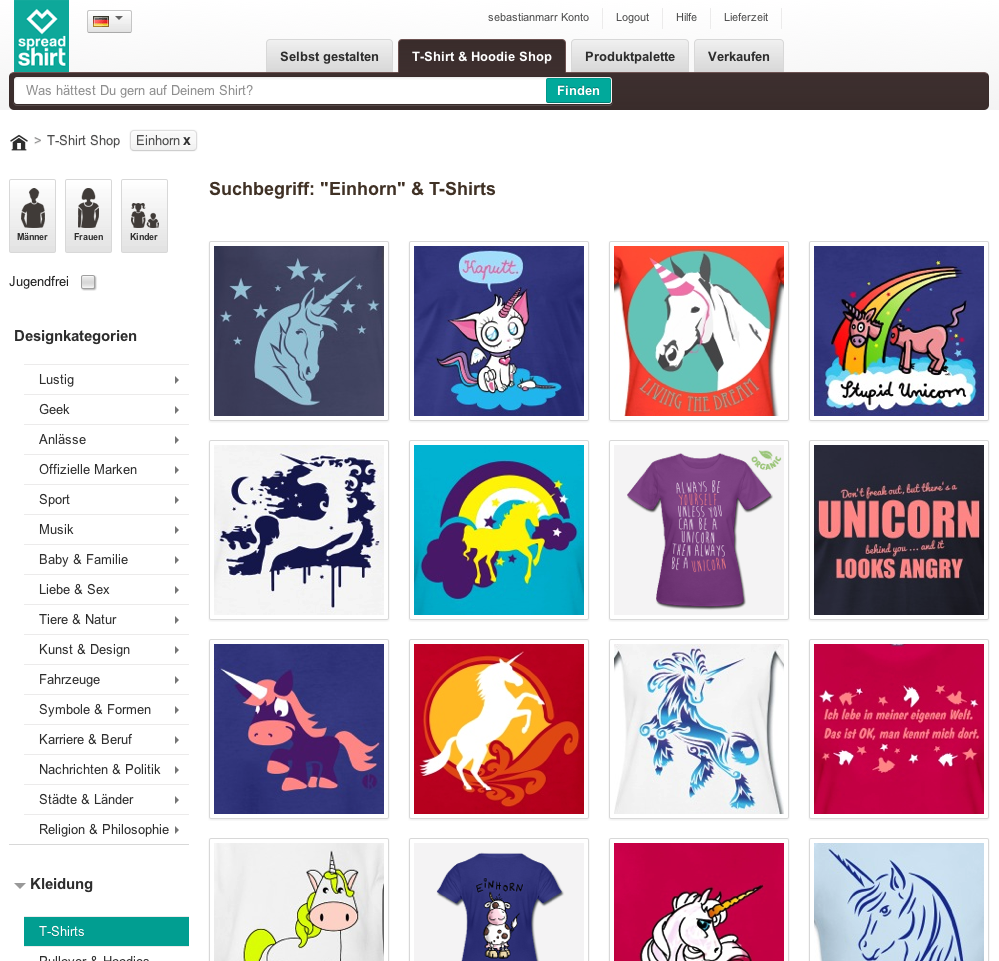
\includegraphics[width=0.9\textwidth]{search_result}
\caption{Suchergebnisseite}
\label{fig:search_result}
\end{figure}

Aufgrund der kürzlichen Einführung des Clicktracking-Systems wurde im Kontext dieser Arbeit mit den ersten \num{611836} aufgezeichneten Klicks gearbeitet.

\subsection{Datenqualität}

Die Qualität von Daten wird im Allgemeinen unter mehreren Gesichtspunkten beurteilt \cite{hkp2012}. Dazu gehören unter Anderem \emph{Korrektheit}, \emph{Vollständigkeit}, und \emph{Redundanzfreiheit}. Nachfolgend werden die bei Spreadshirt vorhandenen Daten nach diesen Kriterien betrachtet und die Quellen eventueller Fehler \cite[43 ff]{jo2003} diskutiert.

\paragraph{Korrektheit}

Die Korrektheit der Tag-Daten kann an vielen Punkten angezweifelt werden. Das hervorstechende Problem hierbei ist das Auftreten von Spam. Viele Partner versehen ihre Artikel und Designs mit Tags, die nicht den Inhalt beschreiben. Partner versehen ihre Designs und Artikeln mit falschen Tags, damit diese bei populären Suchbegriffen gefunden werden.

Ein weiterer Defekt ist die Inkorrektheit des Attributes \emph{Sprache} der Tags. Die Sprache wird aus der Domain abgeleitet, die der Benutzer, der den Tag eingegeben hat, besucht hat. Viele Partner geben jedoch ihre Tags in mehreren Sprachen ein, um ihre Inhalte besser auffindbar zu machen. Dies führt in der Konsequenz dazu, dass das Attribut Sprache im großen Teil der Tags als falsch angesehen werden kann.

Die Quelle beider Fehler ist also die bewusste Falscheingabe von Informationen, um einen persönlichen Vorteil zu erlangen.
                                                                                                                                                                                                                                                                                                                                                                                                              
\paragraph{Vollständigkeit}

Wie bereits in \ref{tag-system} beschrieben, fehlen in den Spreadshirt-Daten der Zeitpunkt und der Benutzer eines Taggings. Dies führt in der Konsequenz dazu, dass Spam schwerer erkannt werden kann. Zwar ist bekannt, wann ein Tag das erste Mal verwendet wurde, alle weiteren Verwendungen des Tags werden haben jedoch keinen Zeitstempel. Der Benutzer, der den Tag angelegt und verwendet hat, kann nur daraus abgeleitet werden, wer den getaggten Artikel angelegt hat.

Die Unvollständigkeit der Daten rührt in erster Linie daher, dass zum Zeitpunkt der Implementierung des Tag-Systems noch nicht bedacht wurde, dass die fehlenden Attribute später nützlich sein können.

\paragraph{Redundanzfreiheit}

Bedingt durch die Form der Dateneingabe besteht für das Vokabular des Tag-System ein großes Potential für redundante Daten. Da eingegebene Tags durch einen Separator getrennt eingegeben werden müssen, besteht hier Potential zur Fehleingabe. Wird der falsche Separator verwendet, werden die eigentlich getrennten Tags als eine einzige Entität abgespeichert.

Technisch kann jeder Tag genau ein Mal in der Datenbank vorkommen. Jedoch führen Rechtschreibfehler, unterschiedliche Groß- und Kleinschreibung, verschiedene Arten zusammengesetzte Wörter zu schreiben, Leerräume vor, nach und zwischen Wörtern eines Tags und Tippfehler dazu, dass das gleiche Wort mehrfach in der Datenbank gespeichert wurde.

Außerdem führten in der Vergangenheit Systemfehler und Implementierungsfehler dazu, dass falsche, nicht druckbare Zeichen in den Tags enthalten waren. Nach Beseitigung der Fehler blieben die fehlerhaften Tags bestehen, so dass bei einer erneuten Eingabe des gleichen Wortes ein neuer Tag in der Datenbank angelegt wurde.

\section{Lösungsansatz}

Die Beziehungen, die zwischen Wörtern und Wortgruppen hergestellt werden können, hängen stark von Umfang, Vielfältigkeit und Qualität der vorhandenen Datenquellen ab. Daher wurde zur Realisierung der Zielstellung ein iterativer Ansatz gewählt.

Die grundsätzliche Lösungsidee besteht in der Erstellung eines Graphen, dessen Knoten Wörter oder Wortgruppen darstellen. Die Kanten zwischen diesen Knoten repräsentieren inhaltliche Beziehungen. Ein erstrebenswertes Ziel ist also ein Graph mit möglichst vielen, duplikatfreien Knoten und vielen, nach inhaltlicher Nähe gewichteten, Kanten. Die hohe Knotenanzahl kommt zum Tragen, um möglichst alle Suchbegriffe und Themen des Anwendungsgebietes abzubilden. Kantenanzahl und -gewichte spielen dann eine Rolle, wenn nach den inhaltlich nächsten Nachbarn eines Knotens gesucht wird.

Um einen solchen Graphen zu erstellen, ist eine Grundmenge von Daten nötig. Diese Grundmenge stellen die Daten des Tag-Systems (\ref{tag-system}) von Spreadshirt dar. Die bereinigten Tags stellen die Knotenmenge dar. Die Kanten werden mittels Kookkurenz ermittelt.

Um die Qualität des Graphen danach schrittweise zu verbessern, werden daraufhin im Laufe der Arbeit weitere externe und interne Datenquellen integriert. Hierbei werden, soweit möglich, ebenfalls kookkurenzbasierte Ansätze gewählt. Diesem Vorgehen liegt die Annahme zu Grunde, dass oft gemeinsam auftauchende Begriffe auch eine inhaltliche Nähe zueinander aufweisen.

Bei jeder neuen Datenquelle muss zunächst die Bereinigung, Integration, Reduktion und Transformation der Daten durchgeführt werden \cite{hkp2012}. Diese Schritte gewährleisten die Datenqualität des Ergebnisgraphen.

Zusammengefasst bedeutet dies, dass abgeleitet von der vorhandenen Knotenmenge weitere Graphen aus anderen Datenquellen erstellt und diese dann in den ursprünglichen Graphen überführt werden. Dies führt einerseits unter Umständen zu einer Erweiterung der Knotenmenge und andererseits zu neuen Kanten mit neuen Gewichten.

Die gewichtete Kombination mehrerer Kanten zwischen zwei Knoten des Graphen stellt also im Ergebnis die inhaltliche Nähe der Begriffe dar, die durch die Knoten repräsentiert werden. Somit muss des weiteren eine geeignete Gewichtung der Kantentypen gefunden werden. Dies ist aufgrund der Natur des Problems nur mit Hilfe von menschlicher Bewertung möglich. Diese Optimierung kann somit gleichzeitig mit der Evaluation statt finden.

Um den Lösungsansatz technisch umzusetzen, soll wenn möglich das Programmiermodell MapReduce \cite{dg2004} eingesetzt werden, da dieses die Skalierung des Vorgehens auf beliebige Datenmengen ermöglicht. Speziell die Erstellung von Kookkurenzgraphen kann deutlich von der Verwendung dieses Verfahrens profitieren.

In den nachfolgenden Kapiteln werden die Umsetzung dieses Lösungsansatzes und die Ergebnisse detailliert beschrieben.
\chapter{Erstellung von Kookkurenzgraphen}

Das folgende Kapitel beschreibt detailliert die Erstellung von Kookkurenzgraphen. Dabei werden die Grundprinzipien erläutert, die existierenden Ähnlichkeitsmaße diskutiert und die algorithmische Umsetzung mittels MapReduce dargestellt.
\chapter{Datenmodell}

Im folgenden Kapitel wird das Datenmodell des im Rahmen dieser Arbeit erstellten Graphen beschrieben.

\begin{figure}
\label{fig:graph_model}
\begin{center}
    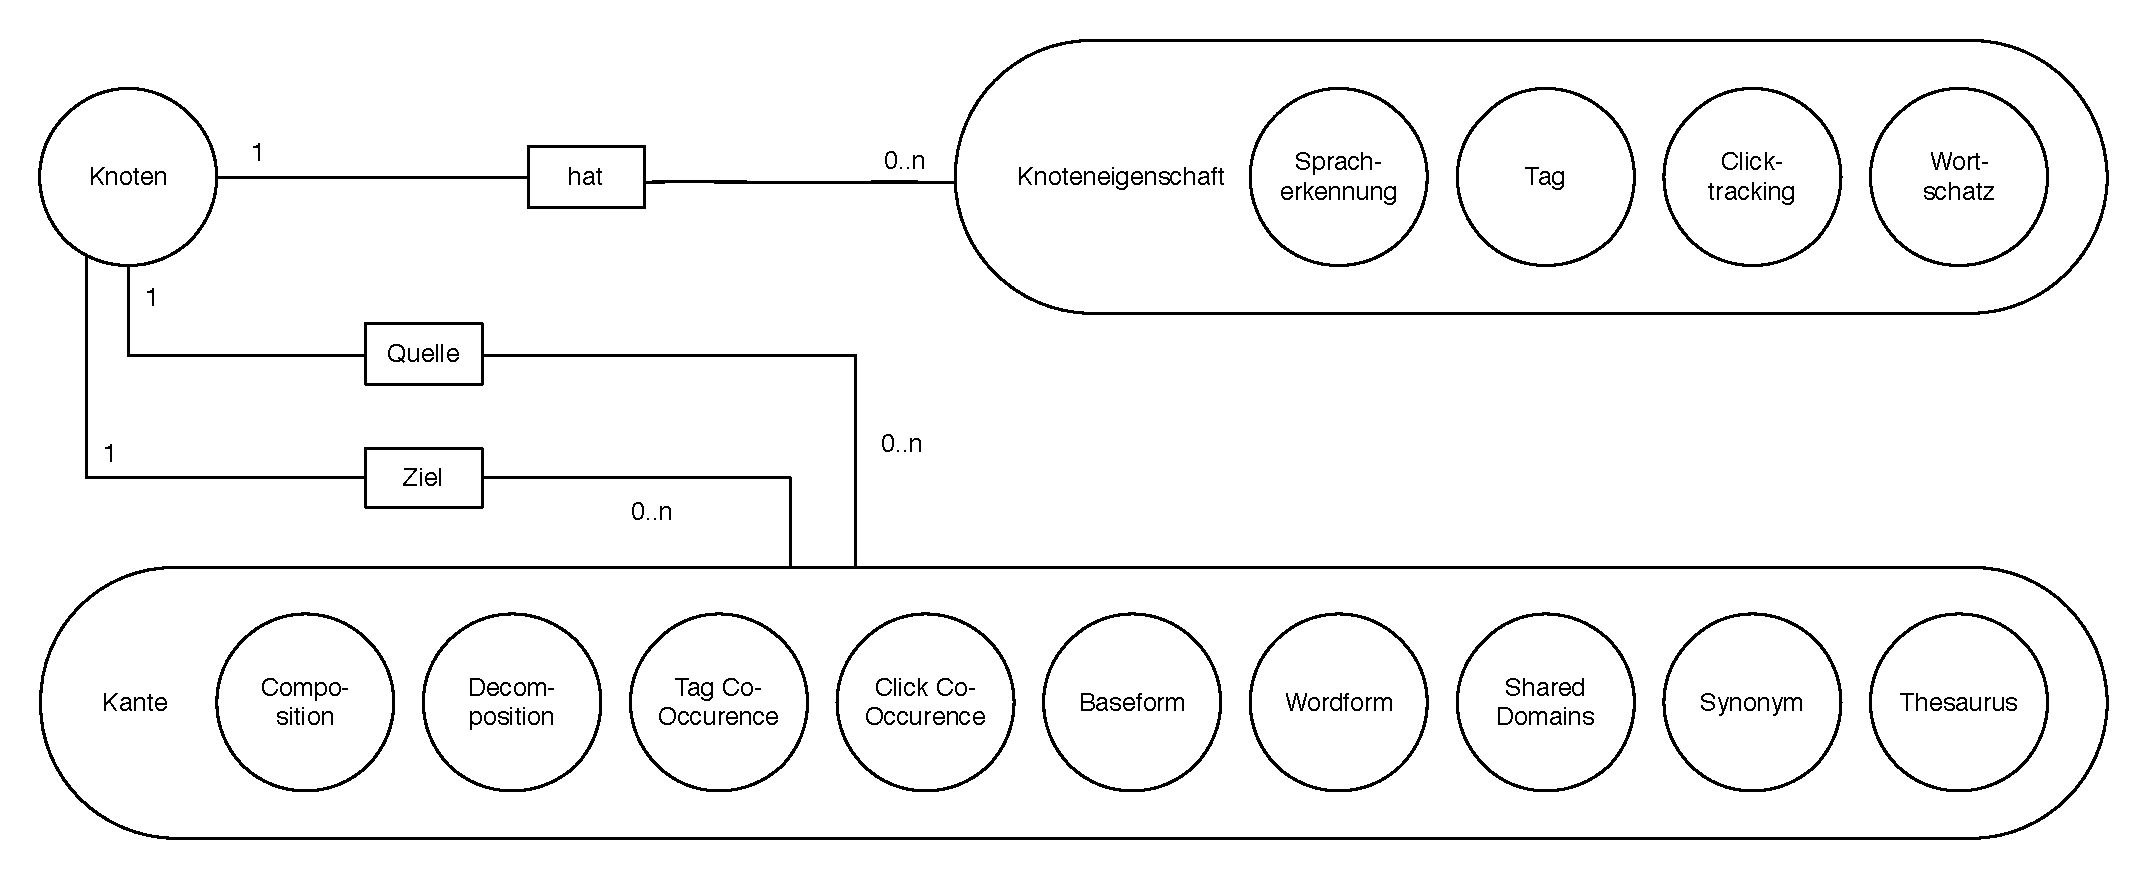
\includegraphics[width=1\textwidth]{graph_model}
\end{center}
\caption{Datenmodell des Graphen als Entity-Relationship-Diagramm}
\end{figure}
\chapter{Externe Datenquellen}

Um den erstellten Graphen aufzuwerten, bietet sich die Integration externer Datenquellen an. Das folgende Kapitel beschreibt die im Rahmen dieser Arbeit verwendeten Datenquellen und deren Integration in den Graphen näher. Konkret handelt es sich dabei um die Google Translate API zur automatischen Spracherkennung sowie das Wortschatz-Projekt der Universität Leipzig zur Ingration von Wortbedeutungen und lingustischen Beziehungen zwischen Begriffen.

\section{Google Translate}

Google bietet im Rahmen seines \emph{Translate}-Services \cite{gt2013} eine kostenpfichtige API für Spracherkennung an. Diese ermöglicht es, die Sprache beliebiger Zeichenketten automatisch erkennen zu lassen. Google stellt hierzu eine REST-API zur Verfügung.

Diese Schnittstelle liefert Ergebnisse der Form \((l, c)\), wobei \(l\) die für die Zeichenkette erkannte Sprache und \(c\) einen Konfidenzwert für die Spracherkennung repräsentiert. Der Konfidenzwert liegt dabei im Intervall zwischen \num{0} und \num{1} und stellt die Verlässlichkeit der Spracherkennung dar.

Die Integration der Spracherkennungs-Daten in den Graphen gestaltet sich einfach. Dazu werden die durch die bereits vorhandenen Knoten repräsentierten Zeichenketten extrahiert und als Eingabedaten für die Spracherkennungs-API verwendet. Die Ergebnisse werden abgespeichert, um weitere kostenpflichtige Abfragen zu vermeiden.

Eine Bereinigung der Ergebnisse ist nicht erforderlich. Somit müssen die Ergebnisse lediglich in den Ausgangsgraphen integriert werden. Die Spracherkennung an sich bringt keine Ähnlichkeitsbeziehungen mit sich, sondern verbessert gegebenenfalls nur die Knotenauswahl für spätere Operationen.

In der Konsequenz genügt es also, die für die Abfrage verwendeten Knoten mit den Ergbenissen der Spracherkennung zu annotieren. Somit kann dann bei späteren Analysen anhand des Konfidenzwertes abgewogen werden, ob die erkannte Sprache oder die eventuell schon am Knoten vorhandene Sprache verwendet werden soll.

\section{Wortschatz der Universität Leipzig}


\chapter{Systemarchitektur}

\begin{figure}[h]
\label{fig:architecture}
\begin{center}
    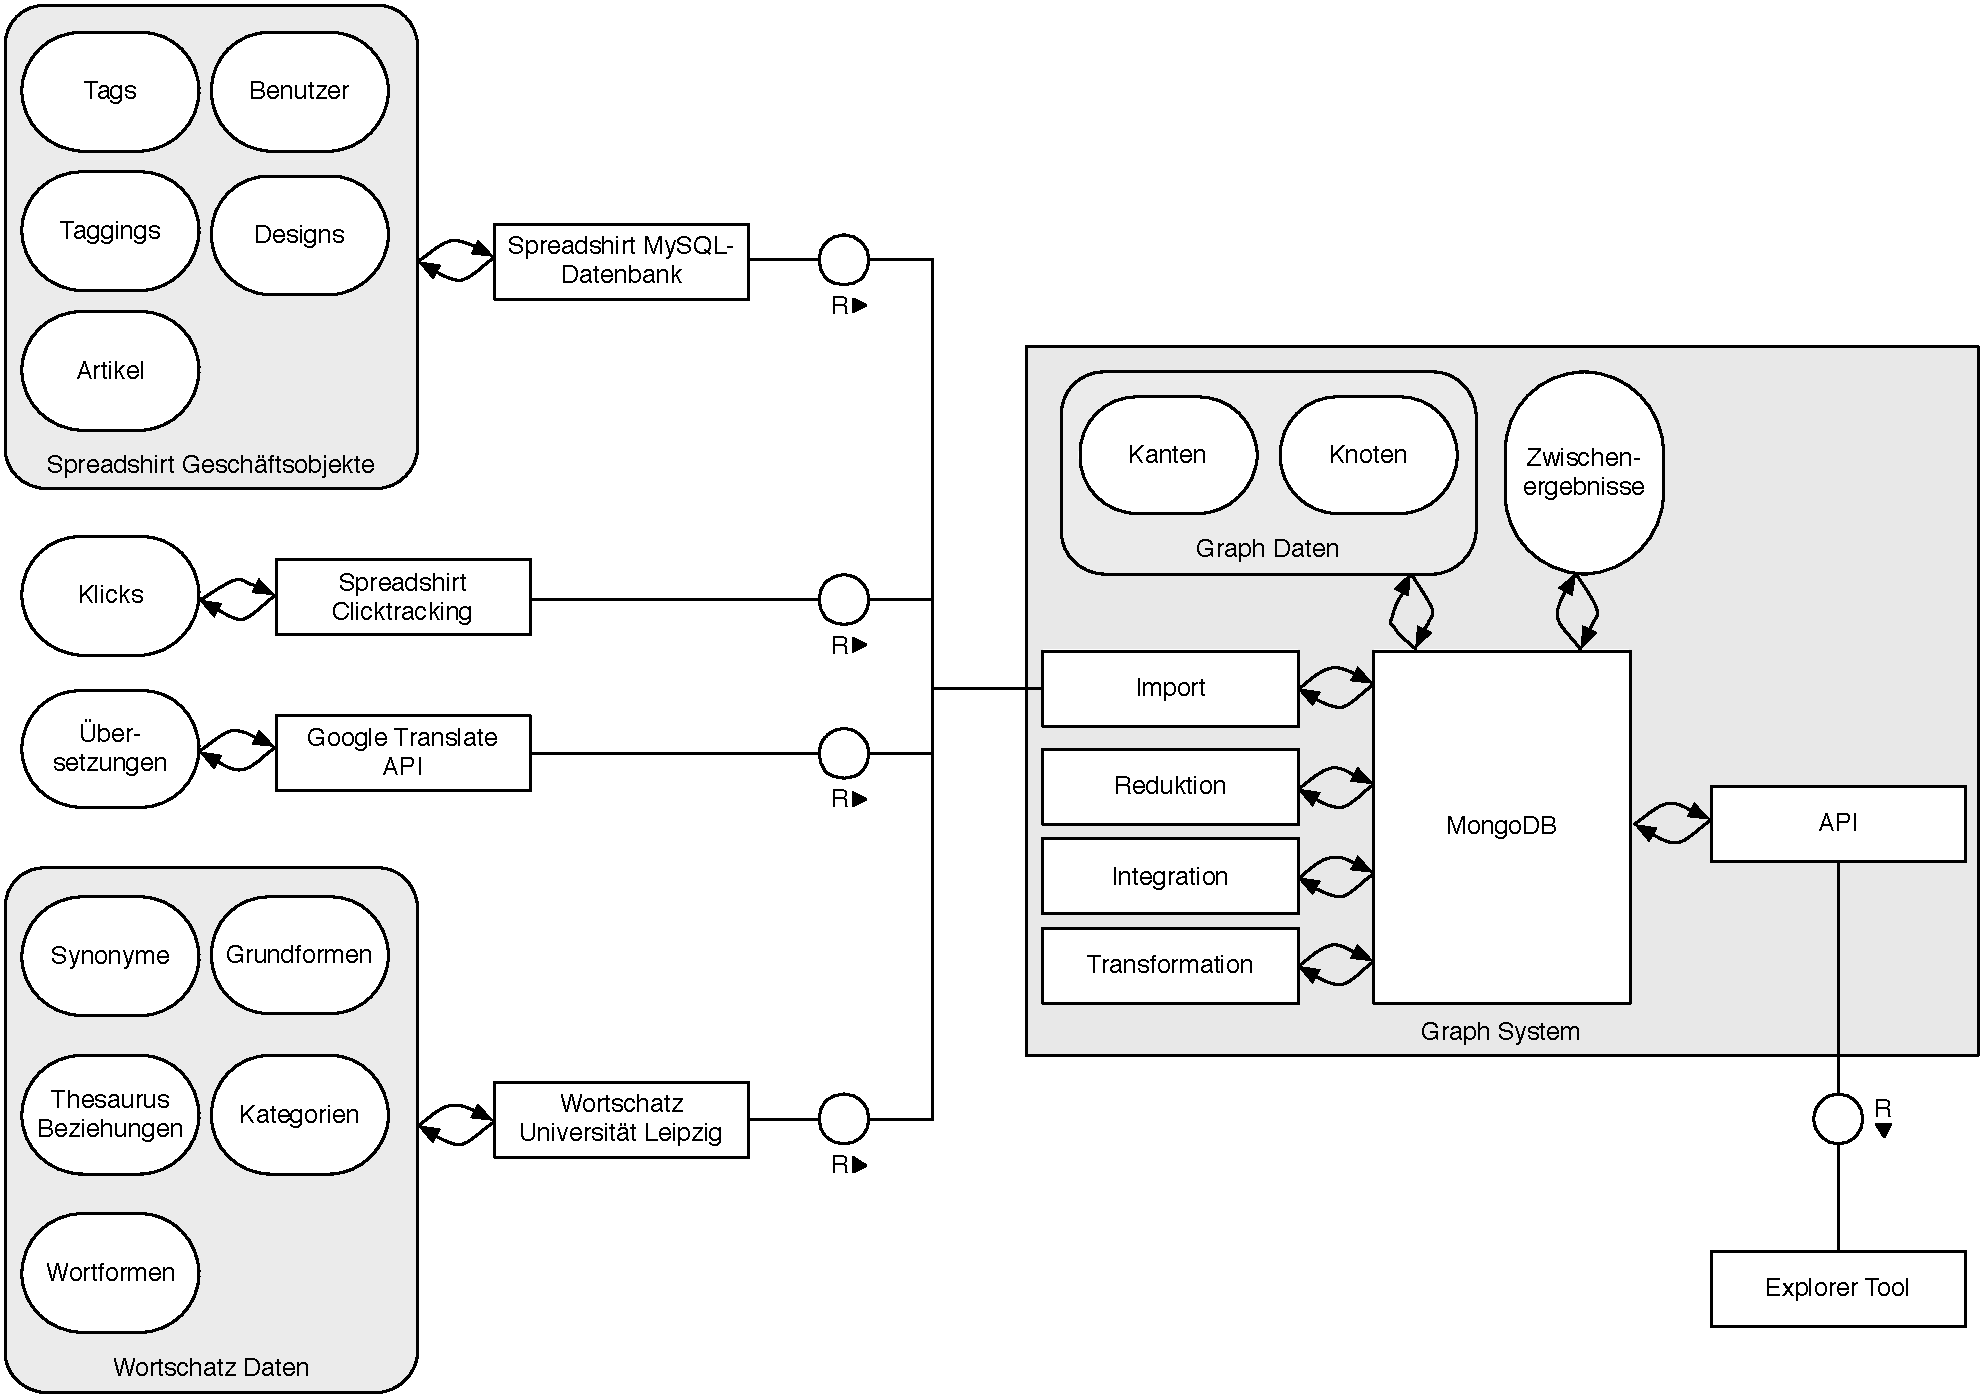
\includegraphics[width=1\textwidth]{architecture}
\end{center}
\caption{Systemarchitektur}
\end{figure}
\chapter{Optimierung und Evaluierung}

Im folgenden Kapitel werden die vorgenommenen Optimierungsmaßnahmen und die damit einhergehende Evaluierung der Ergebnisse der Link Discovery beschrieben. Dazu gehören der gewählte Ansatz zur Optimierung, eine Erläuterung evolutionärer Algorithmen und deren Einsatz zur Optimierung sowie die Darstellung und Auswertung der Ergebnisse.

\section{Optimierung}

Zuerst muss definiert werden, welcher Aspekt genau optimiert werden soll. Die in Kapitel \ref{link_discovery} beschriebenen Schritte haben einen Graphen erzeugt, in dem neun verschiedene Kantentypen existieren. Diese lauten \emph{Tag-Kookkurenz}, \emph{Klick-Kookkurenz}, \emph{Zusammensetzung}, \emph{Zerlegung}, \emph{Wortform}, \emph{Grundform}, \emph{Synonym}, \emph{Kategorie-Kookkurenz} und \emph{Thesaurus-Beziehung}.

Werden nun inhaltlich relevante Nachbarn zu einem gegebenen Begriff gesucht, müssen alle ausgehenden Kanten des entsprechenden Knotens nach Relevanz geordnet werden. Dazu muss jede Kante ein Kantengewicht besitzen. Die Addition aller Kantengewichte zwischen zwei Knoten stellt somit das Maß für ihre Nähe dar.

Die Kanten vom Typ Kookkurrenz besitzen bereits aufgrund der angegebenen Kookkurrenzmaße Kantengewichte. Jedoch muss hierbei festgelegt werden, welches Maß für das Kantengewicht herangezogen werden und in welchem Verhältnis zu den Gewichten anderer Kantentypen es stehen soll.

Somit hängt die Berechnung der Relevanz zwischen zwei Knoten von zwölf Parametern ab. Jedem Kantentyp muss ein Gewicht zugewiesen und außerdem muss eine Auswahl von drei Kookkurrenzmaßen getroffen werden. Die Optimierung und Evaluierung dieser berechneten Relevanz ist Gegenstand dieses Kapitels.

Die Einschätzung, ob die Ordnung der Nachbarn eine Ordnung der Relevanz zum Ausgangsbegriff darstellt, kann dabei nicht automatisch, sondern nur von Menschen, getroffen werden. Somit stellt die Bewertung einer bestimmten Gewichtung der Kanten auch eine Evaluierung der Kantentypen dar.
Generell kann außerdem nicht davon ausgegangen werden, dass eine einmal gefundene Gewichtung der Kanten für alle Knoten des Graphen verwertbare Ergebnisse erzeugt. Daher sollte die Optimierung nicht global, sondern für jeden Knoten einzeln erfolgen. Aufgrund der hohen Knotenanzahl wurde sich hierzu auf eine stichprobenartige Auswahl der Knotenmenge beschränkt.

Durch die Notwendigkeit menschlicher Beteiligung und der großen Anzahl an Parametern ist eine Optimierung mittels des Ausprobierens aller Fälle nicht möglich. Außerdem kann die Einschätzung, welche Kantengewichtungen relevante Ergebnisse erzeugen, stark von Mensch zu Mensch variieren. Stattdessen muss zur Optimierung ein Ansatz gefunden werden, der sich einer, für den Großteil der Personen, optimalen Gewichtung möglichst nähert. 

Im Rahmen dieser Arbeit wurde aus den genannten Gründen ein Optimierungsansatz mittels interaktiver evolutionärer Algorithmen gewählt. Die Grundlagen evolutionärer Algorithmen und die gewählte Implementierung werden in den folgenden Abschnitten beschrieben.

\section{Evolutionäre Algorithmen}

Als evolutionäre Algorithmen wird eine Klasse von Optimierungsverfahren bezeichnet, deren Funktionsweise an die Evolution natürlicher Lebewesen angelehnt ist. Sie versuchen, Probleme durch die Simulation von Evolution mittels der Auswahl der erfolgreichten Individuen zu lösen. Dabei kommen ebenfalls aus der Biologie entlehnte Mechanismen wie Mutation und Rekombination zum Einsatz, um iterativ eine Population von Lösungskandidaten zu verbessern \cite{tw2008}.

Es handelt sich dabei um heuristische Algorithmen, die das Finden einer optimalen Lösung nicht garantieren können.

Grundsätzlich folgt das Vorgehen dabei einem Kreislauf mit den Komponenten \emph{Evaluierung}, \emph{Selektion} und \emph{Reproduktion}. Nach Generierung einer anfänglichen Population (\emph{Initalisierung}) wird dieser Kreislauf so lange durchlaufen, bis ein vorher definiertes Abbruchkriterium eintritt. Ein Durchlauf wird dabei als \emph{Generation} bezeichnet. Das Abbruchkriterium kann beispielweise ein bestimmter Schwellwert für die Güte der Lösung oder eine feste Anzahl von Generationen sein. Der beschriebene Ablauf ist in Abbildung \ref{fig:evo_basic} dargestellt.

\begin{figure}
\centering
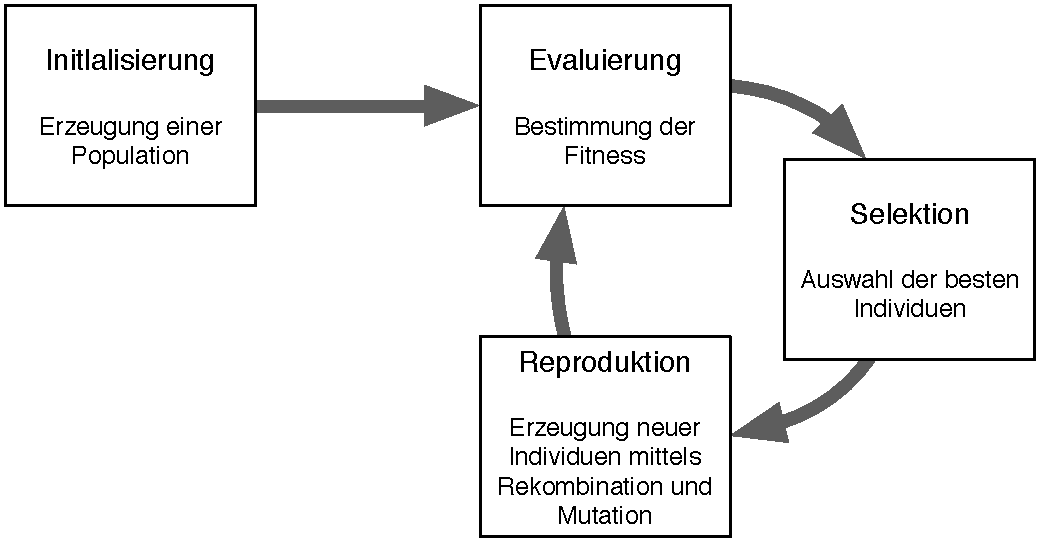
\includegraphics[width=0.8\textwidth]{evo_basic}
\caption{Ablauf evolutionärer Algorithmen}
\label{fig:evo_basic}
\end{figure}

Die einzelnen Komponenten eines evolutionären Algorithmus werden im Folgenden beschrieben. Die Definitionen folgen dabei im Wesentlichen denen von \textcite{tw2008}.

\paragraph{Initialisierung}

Die Population \(P\) stellt eine Menge von Lösungskandidaten dar. Ein Lösungskandidat \(i\) wird dabei als \emph{Individuum} bezeichnet und durch seinen \emph{Genotyp} repräsentiert. Der Genotyp ist die kodierte Repräsentation aller Variablen, die den Lösungskandidaten spezifizieren. Die Variablen werden \emph{Gene} genannt. Im Initlaisierungsschritt werden Lösungskandidaten erzeugt, die die Startpopulation des evolutionären Algorithmus bilden. Die Gene jedes Individuums werden dabei üblicherweise zufällig gewählt.

\paragraph{Evaluierung}

Der Evaluierungsschritt dient zur Bestimmung der \emph{Fitness} der Individuen, die noch in der Population enthalten sind. Die Fitness stellt dabei einen Wert dar, der die Güte der durch das Individuum repräsentierten Lösung bezüglich der Problemstellung beschreibt. Die Fitness kann dabei, je nach Optimierungsproblem, entweder absolut oder bezüglich der anderen Individuen der Population bestimmt werden. Somit lässt sich die Funktion zur Bestimmung der Fitness auf die Form \(fitness(i, P)\) generalisieren.

\paragraph{Selektion}

Im Selektionsschritt werden die fittesten Individuen der Population ausgewählt. Alle nicht ausgewählten Lösungskandidaten werden verworfen. Die Selektion kann dabei als Funktion der Form \(select(P, f, s)\) dargestellt werden, wobei \(s\) eine festgelegte Anzahl von Individuen darstellt, die ausgewählt werden sollen.

\paragraph{Reproduktion}

Die Reproduktion dient dazu, aus den im Selektionschritt ausgewählten Individuen neue Lösungskandidaten zu erzeugen. Dabei werden üblicherweise die Operationen \emph{Rekombination} und \emph{Mutation} verwendet. Eine Rekombination erzeugt dabei, analog zur Biologie, aus zwei Elternindividuen ein neues Kindindividuum. Sie lässt sich dabei als Funktion der Form \(i_n = recombine(i_a, i_b)\) darstellen, wobei \(i_n\) das neue Individuum und \(i_a\) und \(i_b\) die Elternindividuen darstellen. Eine Mutation erzeugt ein neues Individuen durch die Modifikation eines anderen und ist daher durch die Funktion \(i_n = mutate(i_a)\) spezifiziert.

In der Literatur \cite{kw2007, tw2008, dj2006} finden sich für Selektion, Mutation und Rekombination Standardverfahren, die in Hinblick auf das zu lösende Optimierungsproblem ausgewählt werden können. Wie die beschriebenen Schritte des evolutionären Algorithmus für die Optimierung der Link Discovery implementiert wurden, wird im folgenden Abschnitt beschrieben.

\section{Umsetzung}

Nachdem im vorhergehenden Abschnitt die Grundlagen und Komponenten evolutionärer Algorithmen beschrieben wurden, werden im Folgenden die für die Optimierung der Link Discovery-Ergebnnise angewendeten Methoden erläutert.

Zunächst soll die Methode zur Auswahl der Stichproben erläutert werden. Insgesamt wurden fünfzehn Knoten ausgewählt, deren Beziehungen optimiert werden sollen. Die Auswahl der Knoten richtete sich dabei nach der Popularität von Suchbegriffen auf der Spreadshirt-Plattform. Dazu wurden alle Begriffe mit mehr als eintausend Suchen herangezogen und diese nach Häufigkeit der Suchen geordnet. Daraus wurden zufällig je fünf Begriffe bis zum unteren Quartil, fünf Begriffe zwischen unterem und oberen Quartil und fünf Begriffe über dem oberen Quartil ausgewählt. Die ausgewählten Begriffe, deren Kantengewichtungen lokal optimiert werden sollen, lauten: \emph{Kopfkissenbezug}, \emph{Student}, \emph{Volkswagen}, \emph{Marathon}, \emph{Wow}, \emph{Krankenschwester}, \emph{Mountainbike}, \emph{Hammer}, \emph{Polska}, \emph{Regenbogen}, \emph{Minecraft}, \emph{Kind}, \emph{Dubstep}, \emph{Leipzig} und \emph{Valentinstag}.

Ziel dieser Auswahl war, eine möglichst vielfältige Verteilung der einzelnen Kantentypen zu erreichen, aus welcher sich nach Durchführung der Optimierung möglicherweise Erkenntnisse ableiten lassen, ob die Optimierung nur lokal oder auch global druchgeführt werden kann.

\section{Auswertung der Ergebnisse}
\chapter{Schlussbetrachtung}
\label{summary}

In dieser Masterarbeit wurde ein Verfahren und dessen praktische Durchführung zum Finden von Zusammenhängen zwischen Begriffen, die \emph{Link Discovery}, beschrieben. Die Basis dafür stellten die Daten eines Tagging--Systems dar. Dazu wurden Tagging--Systeme grundlegend erläutert, deren Datenmodell definiert und die grundlegenden Unterschiede zwischen Folksonomies und geschlossenen Tagging--Systemen herausgearbeitet. Die Eigenschaften des im späteren Verlauf verwendeten Tagging--Systems von Spreadshirt wurden beschrieben und dessen Datenqualität in Hinblick auf Korrektheit, Vollständigkeit und Redundanzfreiheit diskutiert. Außerdem wurden die zu verarbeitenden Datenmengen definiert.

Für die Durchführung der Link Discovery wurde ein Framework definiert, welches die konzeptionelle Grundlage für die spätere Umsetzung darstellt. Dieses Framework modelliert den betrachteten Weltausschnitt, welcher Begriffe, den Kontext von Begriffen und deren Beziehungen untereinander enthält. Dieser Weltausschnitt wurde in eine Graphenrepräsentation überführt. Weiterhin wurde der Prozess der Link Discovery definiert und die einzelnen Schritte erläutert. Diese bestehen in der initialen Erstellung des Weltausschnittes, der Anreicherung durch Mining oder Integration weiterer Datenquellen und der Priorisierung der erzeugten Beziehungen. Die theoretischen Grundlagen von Kookkurrenz zur Beziehungserzeugung wurden definiert und die Berechnung veranschaulicht.

Weiterhin wurden mögliche Datenquellen diskutiert und die für die praktische Durchführung der Link Discovery in dieser Arbeit verwendeten Quellen ausgewählt. Diese bestehen aus dem Tagging-- und Clicktracking--System von Spreadshirt sowie dem Wortschatz der Universität Leipzig. Zur Priorisierung der erzeugten Beziehungen wurden evolutionäre Algorithmen erläutert und deren Einsatz im Rahmen der Priorisierung definiert.

Diese theoretischen Grundlagen wurden anschließend an konkreten Daten praktisch umgesetzt. Für jede integrierte Datenquelle wurden die Schritte Import, Bereinigung, Reduktion, Transformation in die Graphenrepräsentation und Integration in den Weltausschnitt ausführlich dargestellt und die quantitativen Ergebnisse präsentiert. Zur Anreicherung durch Mining wurde die Zerlegung von Wortgruppen in Einzelwörter erläutert. Im Anschluss wurden die quantitativen Veränderungen der Graphenrepräsentation nach jedem Link--Discovery--Schritt dargestellt und diskutiert. Nachdem alle Datenquellen integriert waren, wurde die praktische Umsetzung der Priorisierung der Beziehung mittels evolutionärer Algorithmen dargestellt und die Ergebnisse präsentiert.

Weiterhin wurden die Anforderungen an ein technisches System, welches die Link Discovery implementiert, formuliert und deren Umsetzung im Rahmen dieser Arbeit beschrieben. Dazu gehören die Wahl des Datenbanksystems MongoDB, die Implementierung der Komponenten in der Programmiersprache JavaScript und die Beschreibung von Kookkurrenzberechnung mittels des Programmiermodells MapReduce.

Die Ergebnisse dieser Arbeit stellen die Grundlage für weitere mögliche Arbeiten dar. Eine zukünftige Arbeit könnte sich mit der Auswertung der inhaltlichen Qualität der erzeugten Beziehungen beschäftigen. Dazu wird eine gründliche Analyse der integrierten Datenquellen und des Ergebnisses der Link Discovery mit Hilfe menschlicher Beurteilung benötigt.

Weiterhin sind Arbeiten denkbar, die die erzeugten Beziehungen für weitere Analyseverfahren nutzen. So könnten beispielsweise die Beziehungen zum Clustering der Begriffe zu Themen genutzt werden. Werden hierarchische Clusteringverfahren genutzt, können daraus Themenbäume und Topic Maps abgeleitet werden. Diese Themenbäume können sich durch ständige Durchführung der Link Discovery an aktuelle Trends in den Inhalten der betrachteten Website anpassen.

Der Link--Discovery--Prozess könnte durch einen interaktiven Trainingsschritt erweitert werden. In diesem Schritt wird die Beurteilung der Beziehungen durch Benutzer nicht nur zur Priorisierung, sondern zur direkten Veränderung des Weltausschnittes genutzt. Dabei werden Kanten eingefügt, die explizite statt nachträglich hergestellte Zusammenhänge beschreiben. Außerdem könnten durch manuellen Eingriff fehlerhafte Beziehungen gelöscht werden.

Insgesamt stellt das in dieser Arbeit beschriebene Framework eine gute Basis für Erweiterungen und neue Implementierungen dar. Das Verfahren ist flexibel und leistungsfähig genug, um auch auf anderen Datenbeständen gute Ergebnisse erzielen zu können. Durch Integration anderer Datenquellen und neuer Analyseverfahren kann die Qualität der gefundenen Zusammenhänge stetig verbessert werden. Die konkret erzeugten Daten bieten eine gute Grundlage für weitere Auswertungen und praktische Anwendungen.

% \nocite{*}
\printbibliography 

\end{document}